{\chapter{Literature review}
An overview of the Total Hip Arthroplasty is given in section 3.1. After this, in section 3.2 the indications for THA are listed. Section 3.3 elaborates on preoperative templating and section 3.4 on the most used surgical approaches. Reasons for failure of THA are stated in section 3.5. During the surgery range of motion is measured, section 3.6 explains the importance of this and the limitations and shortfalls of the tools used for this. With this information, a new set of requirements is made for a new device using Inertial Measurement Units (IMU). Section 3.7 elaborates on the working principle of the IMU and how it can be used to measure the range of motion during THA.     
\section{The principle of Total Hip Arthroplasty}
Total Hip Arthroplasty (THA) is a procedure where a defective hip joint with pain symptoms or functional impairment caused by degenerative bone or joint diseases like osteoarthritis is replaced by a hip prosthetic. A modular hip prosthesis design consists of an acetabular cup, femoral head and stem~\cite{holzwarth2012total} as shown in Figure 1. Polyethylene is used for the acetabular cup and consists of a shell and liner. The shell is anchored into the pelvis joint and has a liner inserted that functions as a load-bearing layer between the femoral head and the shell. The femoral head is attached to the stem and is inserted in the femur. Fixation of the stem can be done by using acrylic bone cement or by a press fit~\cite{holzwarth2012total}. Cemented stems must be stiff and have a smooth surface to avoid cement fracture. Non-cemented stems have coated surfaces where newly-formed bone tissue can grow. The materials used for the prosthesis must have low friction and withstand wear and oscillating mechanical load. Materials that can be used are stainless steel, cobalt-chromium-molybdenum or titanium-alloys~\cite{holzwarth2012total}. The customizable design allows different materials with different properties.
\begin{figure}[ht]
    \centering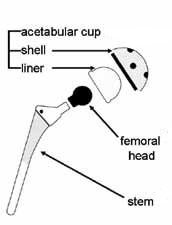
\includegraphics[width=0.5\linewidth]{schematic_scheme_hip_prosthetic.jpg}
\end{figure}
\begin{figure}[ht]
	\centering
	\begin{subfigure}{0.5\linewidth}
		\centering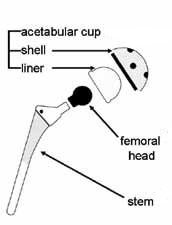
\includegraphics[width=1\linewidth]{schematic_scheme_hip_prosthetic.jpg}
		\caption{\label{fig:fig1}}
	\end{subfigure}%
	\begin{subfigure}{0.5\linewidth}
		\centering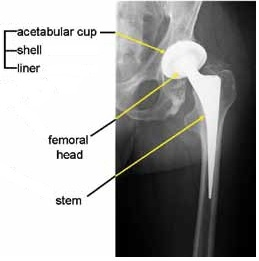
\includegraphics[width=1\linewidth]{Xray_hip_prosthetic.jpg}
		\caption{\label{fig:fig2}}
	\end{subfigure}  
	\caption{\subref{fig:fig1} shows a schematic scheme of the prosthetic and~\subref{fig:fig2} a X-ray image of the prosthesis~\cite{holzwarth2012total}}
\end{figure}
	
